\chapter{Machines à Vecteurs de Support (SVM)}
\section{Introduction et Contexte Historique}
Les Support Vector Machines (SVM) ont été développées par \textbf{Vladimir Vapnik}. Bien que l'idée remonte aux années 60, Vapnik a fait face à des rejets initiaux (notamment 3 papiers refusés à NIPS en 1992) avant de connaître le succès aux Bell Labs grâce à l'introduction du premier noyau non-linéaire (polynomial d'ordre 2) pour la reconnaissance de chiffres manuscrits.

\subsection{Objectif de la Classification Supervisée}
La classification consiste à construire une fonction $C(X)$ à partir de prédicteurs $X$ pour prédire une réponse qualitative $Y$ appartenant à un ensemble de classes $\mathcal{C}$.
\begin{itemize}
    \item \textbf{Variables Qualitatives :} Valeurs dans un ensemble non ordonné (ex: couleur des yeux, fraude ou non).
    \item \textbf{Probabilités :} Dans certains domaines (assurance), l'estimation de la probabilité d'appartenance à une classe est plus utile qu'une classification brute.
    \item \textbf{Spécificité SVM :} Ils sont nativement conçus pour la prédiction de classe, bien qu'adaptables pour l'estimation de probabilités.
\end{itemize}

\section{Classification et Hyperplan Séparateur}

\subsection{Définition Mathématique}
Un hyperplan $H$ dans un espace vectoriel de dimension $p$ est défini par l'équation:
\begin{equation}
\beta_{0} + \beta_{1}x_{1} + \dots + \beta_{p}x_{p} = 0
\end{equation}
\begin{itemize}
    \item Si $p=2$, l'hyperplan est une simple \textbf{droite}.
    \item Si $\beta_{0}=0$, l'hyperplan passe par l'origine.
    \item Le vecteur $\vec{\beta} = (\beta_{1}, \dots, \beta_{p})^{T}$ est normal à l'hyperplan.
\end{itemize}
L'hyperplan divise l'espace en deux \textbf{demi-espaces}. Le signe de la fonction $f(x) = \beta_{0} + \sum \beta_{j}x_{j}$ indique de quel côté de l'hyperplan se trouve un point $x$.

\begin{figure}[h]
    \centering
    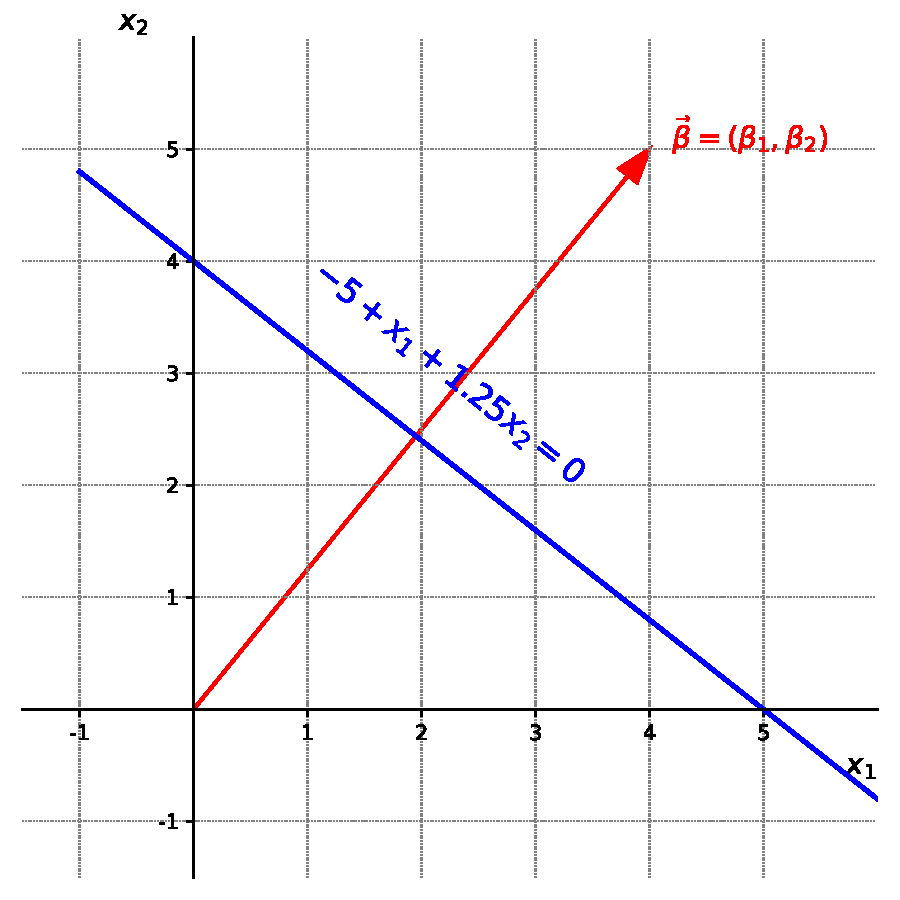
\includegraphics[width=0.45\textwidth]{images/svm_hyperplane.pdf}
    \caption{Exemple d'hyperplan $x_2 = 4 - 0.8x_1$ avec son vecteur normal $\vec{\beta}$}
    \label{fig:svm_hyperplane}
\end{figure}

\subsection{Règle de Décision}
Soit $n$ observations d'entraînement $\vec{x}_{1}, \dots, \vec{x}_{n}$ associées à des classes $y_{i} \in \{-1, +1\}$. Si un hyperplan séparateur parfait existe, il vérifie:
\begin{equation}
y_{i}(\beta_{0} + \beta_{1}x_{i1} + \dots + \beta_{p}x_{ip}) > 0, \quad \forall i=1, \dots, n
\end{equation}

Pour une nouvelle observation $x^*$, on prédit la classe selon le signe de $f(x^*)$:
\begin{itemize}
    \item $f(x^*) > 0 \implies \text{Classe } +1$.
    \item $f(x^*) < 0 \implies \text{Classe } -1$.
\end{itemize}

\section{Le Classifieur à Marge Maximale}

\subsection{Principe}
Parmi l'infinité d'hyperplans séparateurs possibles, on cherche celui qui maximise la \textbf{marge} (le gap) entre les deux classes. C'est l'approche de la "rue la plus large".

\begin{figure}[h]
    \centering
    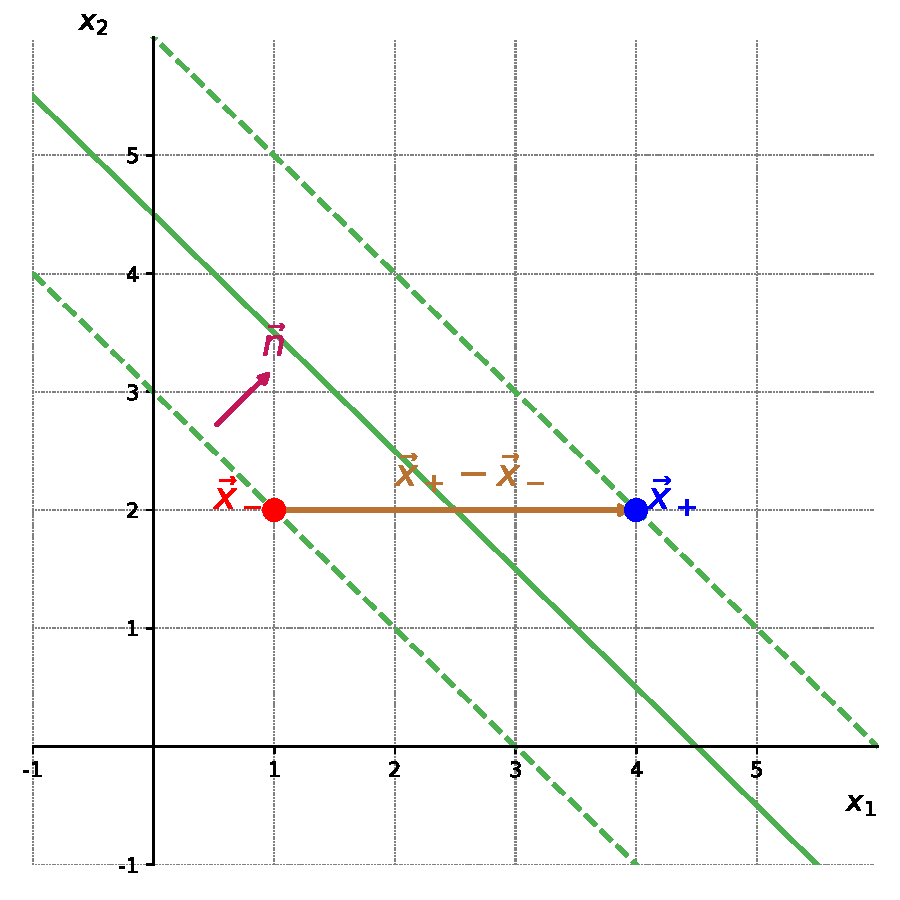
\includegraphics[width=0.45\textwidth]{images/svm_margin_geometry.pdf}
    \caption{Géométrie de la marge maximale entre deux vecteurs supports $\vec{x}_+$ et $\vec{x}_-$}
    \label{fig:svm_margin_geometry}
\end{figure}

\subsection{Optimisation}
Maximiser la largeur globale de la marge \textbf{($\bigstar$ EXAMEN)} $L = \frac{2}{\|\vec{\beta}\|} = \frac{2}{\sqrt{\beta^T \beta}}$ revient à minimiser $\|\vec{\beta}\|$ sous contraintes. Le problème quadratique (QP) s'écrit:
\begin{equation}
\min_{\beta_0, \beta} \frac{1}{2}\|\vec{\beta}\|^{2} \quad \text{s.t.} \quad y_{i}(\beta_{0} + \vec{\beta}^{T}\vec{x}_{i}) \geq 1, \quad i=1, \dots, n
\end{equation}

\begin{figure}[h]
    \centering
    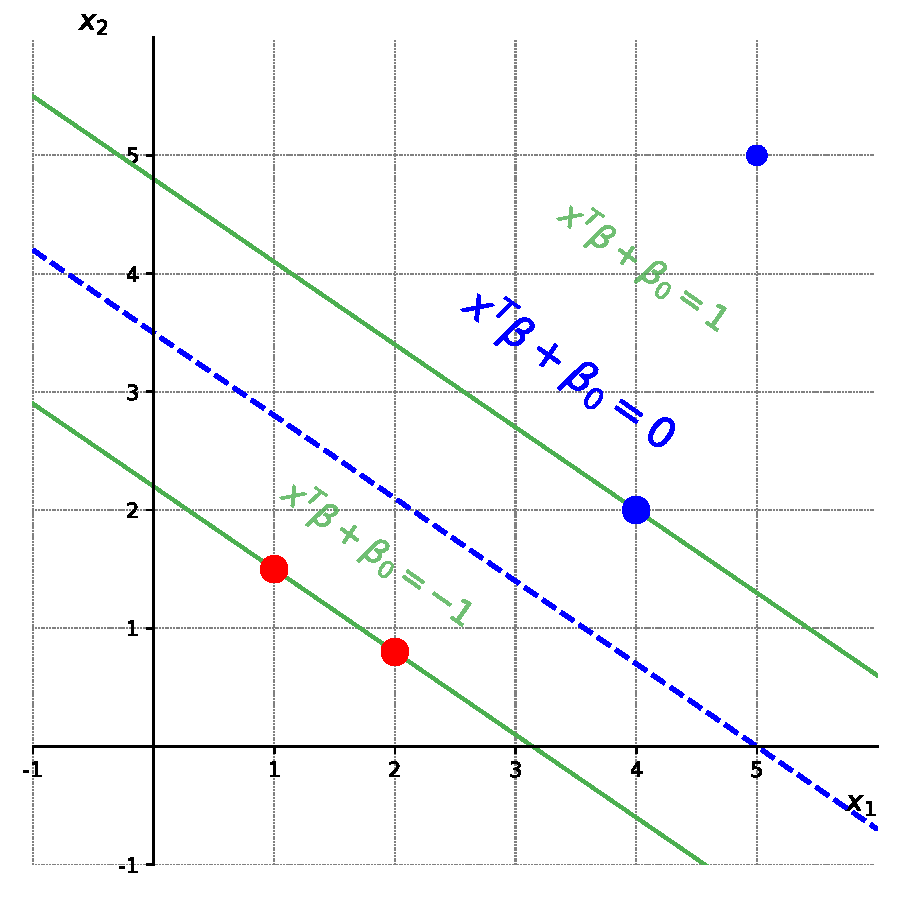
\includegraphics[width=0.45\textwidth]{images/svm_hyperplanes_equations.pdf}
    \caption{Les équations définissant l'hyperplan séparateur (0) et les frontières de marge (+1 et -1)}
    \label{fig:svm_hyperplanes_equations}
\end{figure}

\subsection{Vecteurs Supports et Dualité}
On utilise le \textbf{Lagrangien} pour résoudre ce problème sous contraintes:
\begin{equation}
L = \frac{1}{2}\|\vec{\beta}\|^{2} - \sum_{i=1}^{N} \alpha_{i}[y_{i}(\vec{\beta} \cdot \vec{x}_{i} + \beta_{0}) - 1]
\end{equation}
En annulant les dérivées partielles, on trouve que $\vec{\beta}$ est une combinaison linéaire des échantillons:
\begin{equation}
\vec{\beta} = \sum_{i=1}^{N} \alpha_{i}y_{i}\vec{x}_{i}
\end{equation}
\textbf{Points clés :}
\begin{itemize}
    \item Seuls les points sur la marge (\textbf{Vecteurs Supports}) ont un multiplicateur de Lagrange $\alpha_i > 0$.
    \item L'optimisation et la décision ne dépendent que des \textbf{produits scalaires} entre les paires d'échantillons.
\end{itemize}

\section{Support Vector Classifier (Cas Non-Séparable)}

Dans la réalité, les données sont souvent bruitées ou non linéairement séparables.

\subsection{Variables d'Écart (Slack Variables)}
On introduit $\xi_i \geq 0$ pour autoriser certaines observations à se trouver du mauvais côté de la marge ou de l'hyperplan:
\begin{itemize}
    \item $\xi_i = 0$ : Point bien classé, hors de la marge.
    \item $\xi_i > 0$ : Point ayant dépassé la marge.
    \item $\xi_i > 1$ : Point mal classé (mauvais côté de l'hyperplan).
\end{itemize}

\subsubsection{Le paramètre de coût $C$}
On minimise $\frac{1}{2}\|\beta\|^2 + C \sum \xi_i$. \textbf{($\bigstar$ EXAMEN)}
\begin{itemize}
    \item \textbf{$C$ petit :} On est très tolérant aux erreurs (somme des $\xi_i$ peu pénalisée). La marge s'élargit et autorise davantage d'observations à la violer, conduisant à un modèle plus souple (biais plus fort, variance plus faible).
    \item \textbf{$C$ grand :} On est très sévère quant aux erreurs. La marge se resserre considérablement pour classer correctement le maximum de points d'entraînement, ce qui rapproche le modèle du classifieur à marge maximale (faible biais, variance très forte risquant le sur-apprentissage).
\end{itemize}

\begin{figure}[h]
    \centering
    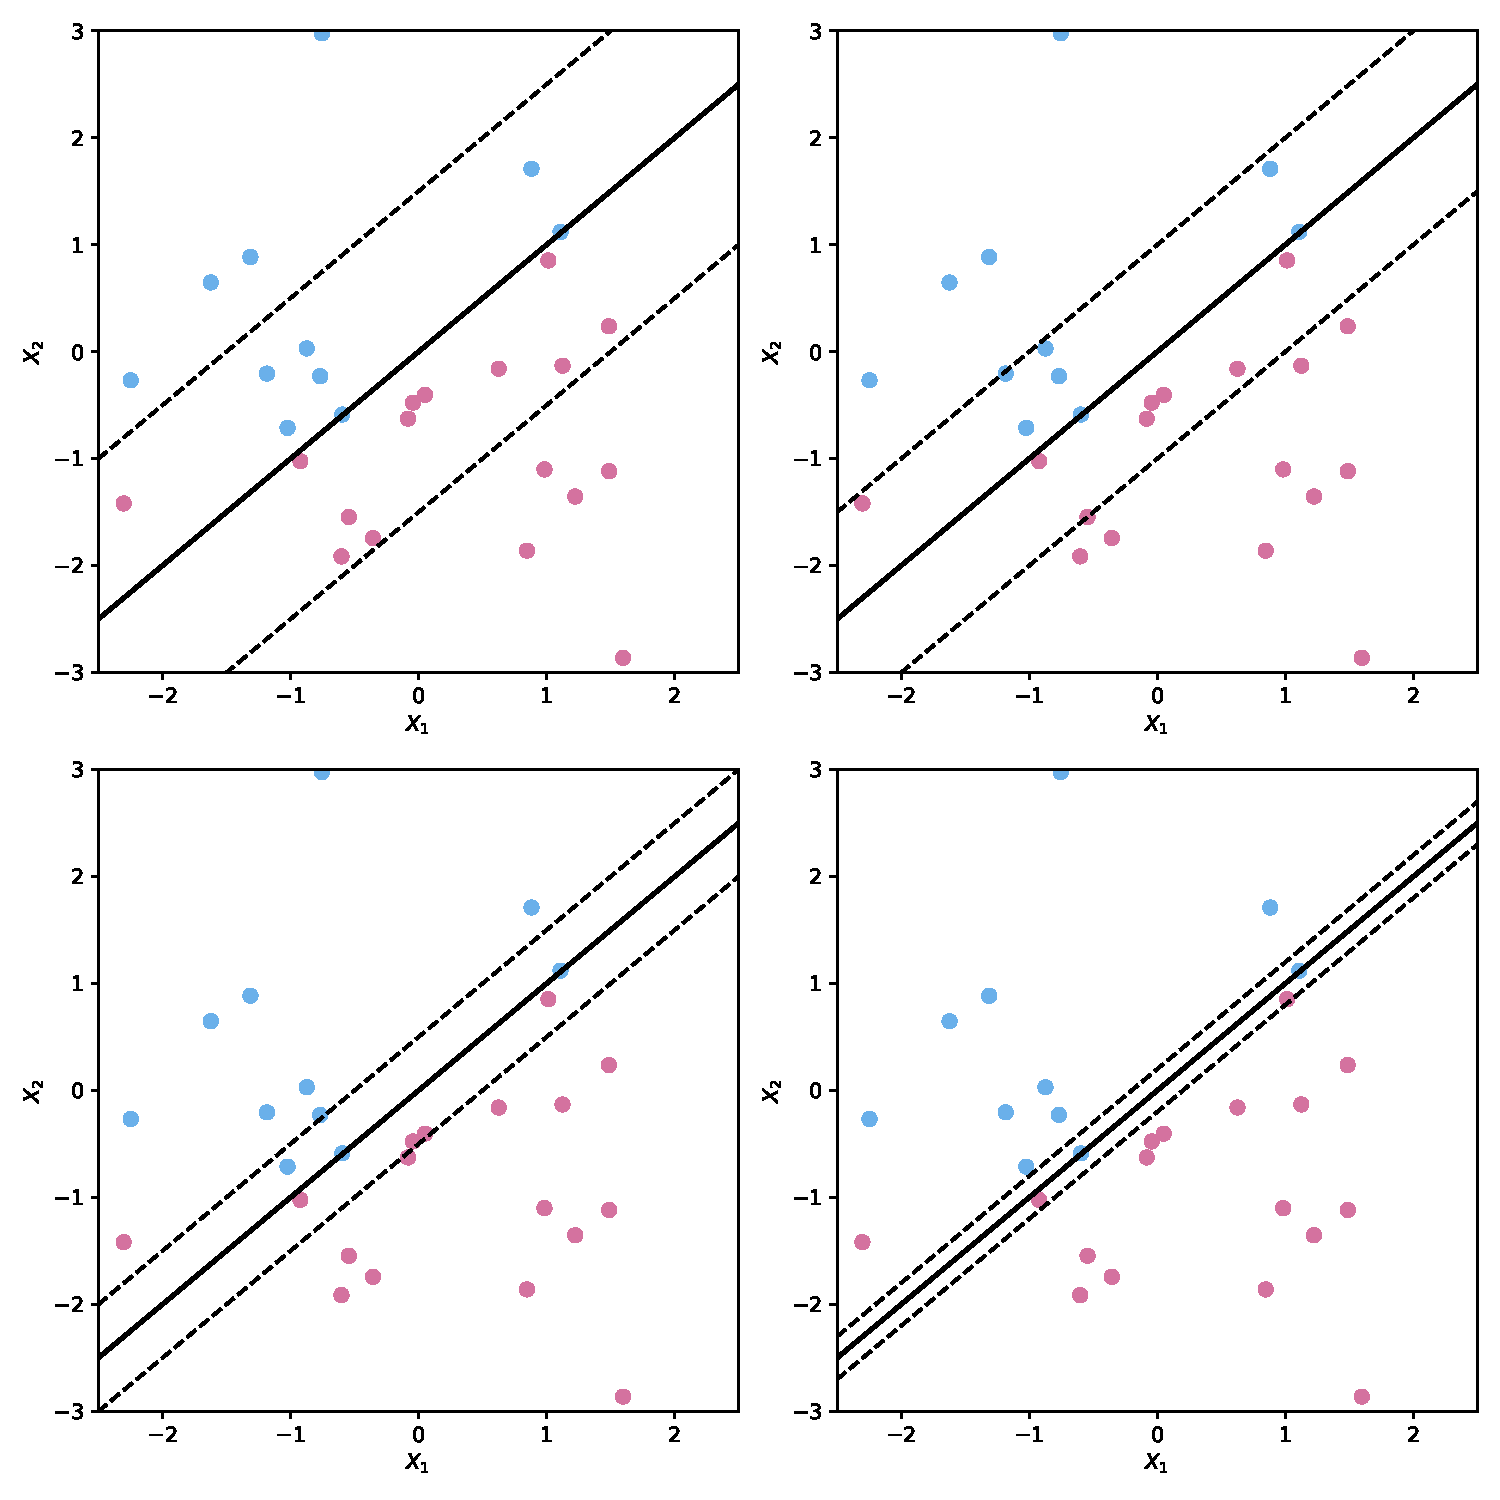
\includegraphics[width=0.7\textwidth]{images/svm_svc_noisy.pdf}
    \caption{Effet de la flexibilité du classifieur (paramètre de coût $C$) sur des données bruitées}
    \label{fig:svm_svc_noisy}
\end{figure}

\subsection{Formulation Duale (Soft Margin) et Résolution Mathématique}
Le passage du problème d'optimisation \textbf{primal} (minimisation avec contraintes) au problème \textbf{dual} (maximisation) repose sur le \textbf{Lagrangien}. Voici le détail de la méthode :

\subsubsection{1. Le problème primal et le Lagrangien}
Le problème d'optimisation \textit{Soft Margin} primal est le suivant :
\begin{equation}
\min_{\beta_0, \beta, \xi} \frac{1}{2}\|\vec{\beta}\|^2 + C \sum_{i=1}^n \xi_i
\end{equation}
Sous les contraintes :
\begin{align}
& y_i(\beta_0 + \vec{\beta}^T \vec{x}_i) \geq 1 - \xi_i, \quad \forall i \\
& \xi_i \geq 0, \quad \forall i
\end{align}

Pour intégrer ces contraintes, on introduit des \textbf{multiplicateurs de Lagrange} $\alpha_i \geq 0$ (pour la première contrainte) et $\mu_i \geq 0$ (pour la positivité des "slack variables" $\xi_i$). Le Lagrangien s'écrit :
\begin{equation}
L(\beta, \beta_0, \xi, \alpha, \mu) = \frac{1}{2}\|\vec{\beta}\|^2 + C \sum_{i=1}^n \xi_i - \sum_{i=1}^n \alpha_i \left[ y_i(\beta_0 + \vec{\beta}^T \vec{x}_i) - 1 + \xi_i \right] - \sum_{i=1}^n \mu_i \xi_i
\end{equation}

\subsubsection{2. Conditions d'optimalité (KKT)}
Pour minimiser ce Lagrangien par rapport aux variables primales ($\beta, \beta_0, \xi$), on annule les dérivées partielles :
\begin{align}
    \frac{\partial L}{\partial \vec{\beta}} &= 0 \implies \vec{\beta} = \sum_{i=1}^n \alpha_i y_i \vec{x}_i \label{eq:beta} \\
    \frac{\partial L}{\partial \beta_0} &= 0 \implies \sum_{i=1}^n \alpha_i y_i = 0 \label{eq:beta0} \\
    \frac{\partial L}{\partial \xi_i} &= 0 \implies \alpha_i + \mu_i = C \label{eq:xi}
\end{align}

\subsubsection{3. Le problème Dual}
En substituant les résultats \eqref{eq:beta}, \eqref{eq:beta0} et \eqref{eq:xi} dans le Lagrangien, les termes dépendant de $\beta_0$ et de $\xi_i$ s'annulent. La fonction (dual) à \textbf{maximiser} ne dépend plus que des multiplicateurs $\alpha_i$ :
\begin{equation}
\max_{\alpha} \sum_{i=1}^n \alpha_i - \frac{1}{2} \sum_{i=1}^n \sum_{j=1}^n \alpha_i \alpha_j y_i y_j \vec{x}_i^T \vec{x}_j
\end{equation}

\textbf{($\bigstar$ EXAMEN) Contraintes finales sur $\alpha_i$ (Box-Constraint) :}
\begin{itemize}
    \item La condition \eqref{eq:beta0} nous donne : $\sum_{i=1}^n \alpha_i y_i = 0$.
    \item Puisque $\alpha_i \geq 0$ et $\mu_i \geq 0$, l'équation \eqref{eq:xi} ($\alpha_i + \mu_i = C$) implique nécessairement la contrainte dite de "boîte" (\textit{Box-Constraint}) sur chaque multiplicateur :
    \begin{equation}
        0 \leq \alpha_i \leq C, \quad \forall i=1, \dots, n
    \end{equation}
\end{itemize}

\subsubsection{4. \textbf{($\bigstar$ EXAMEN)} Variante de Pénalité : Le Soft Margin $L_2$}
Notez que le problème primal présenté précédemment ajoute une pénalité linéaire (Norme $L_1$) sur les erreurs $C \sum \xi_i$. Il existe une variante mathématique classique où l'on utilise une norme $L_2$ sur ces variables d'écart :
\begin{equation}
\min_{\beta_0, \beta, \xi} \frac{1}{2}\|\vec{\beta}\|^{2} + \frac{C}{2} \sum_{i=1}^n \xi_i^2
\end{equation}
Cette variante modifie drastiquement le Lagrangien. Comme $\xi_i^2 \ge 0$, la variable $\xi_i$ porte déjà la positivité, et on omet souvent le terme $-\sum \mu_i \xi_i$. La dérivée par rapport à $\xi_i$ n'est plus $C - \alpha_i - \mu_i = 0$, mais devient une relation proportionnelle $C\xi_i - \alpha_i = 0$, soit $\xi_i = \alpha_i / C$.

\textbf{($\bigstar$ EXAMEN) Formulation Duale exacte de la variante $L_2$ :} En réinjectant $\xi_i$, la fonction objectif ($A_1$) à maximiser et ses contraintes ($A_2$) deviennent formellement :
\begin{equation}
\max_{\alpha} \sum_{i=1}^n \alpha_i - \frac{1}{2} \sum_{i=1}^n \sum_{j=1}^n \alpha_i \alpha_j y_i y_j \vec{x}_i^T \vec{x}_j - \frac{1}{2C} \sum_{i=1}^n \alpha_i^2
\end{equation}
\begin{equation}
\text{s.t.} \quad \sum_{i=1}^n \alpha_i y_i = 0 \quad \text{et} \quad A_2 : 0 \le \alpha_i
\end{equation}
La matrice noyau subit un ajout sur sa diagonale et la contrainte de "boîte" supérieure disparaît (l'écrasement $C$ est absorbé géométriquement par la pénalisation quadratique $-\frac{1}{2C} \alpha_i^2$). Il est essentiel de ne pas confondre les formulations lors de l'examen.

\subsubsection{4. Interprétation des Multiplicateurs (Vecteurs Supports)}
Les conditions de Karush-Kuhn-Tucker (KKT) imposent que le produit multiplicateur $\times$ contrainte est nul à l'optimum (\textit{complementary slackness}) :
\begin{align}
    \alpha_i \left[ y_i(\beta_0 + \vec{\beta}^T \vec{x}_i) - 1 + \xi_i \right] &= 0 \\
    \mu_i \xi_i &= 0
\end{align}
Cela permet de classifier les observations d'entraînement :
\begin{itemize}
    \item \textbf{Points bien classés (hors de la marge) :} $\xi_i = 0 \implies \mu_i > 0 \implies \alpha_i = 0$. Ces points n'influencent pas l'hyperplan.
    \item \textbf{Vecteurs supports sur la frontière de la marge :} $0 < \alpha_i < C$. Par l'équation \eqref{eq:xi}, $\mu_i > 0 \implies \xi_i = 0$. Le point est exactement sur la marge, bien classé.
    \item \textbf{Vecteurs supports mal placés (dans la marge ou du mauvais côté) :} $\alpha_i = C$. Alors $\mu_i = 0$, et donc $\xi_i$ peut être strictement positif ($\xi_i > 0$).
\end{itemize}

\section{Support Vector Machines et Noyaux}

\subsection{Le "Kernel Trick"}
Si les données ne sont pas séparables linéairement dans l'espace d'origine $\mathbb{R}^p$, on les projette dans un espace de dimension supérieure $\mathbb{R}^P$ via une transformation $\phi$ où elles deviennent séparables.

\begin{figure}[h]
    \centering
    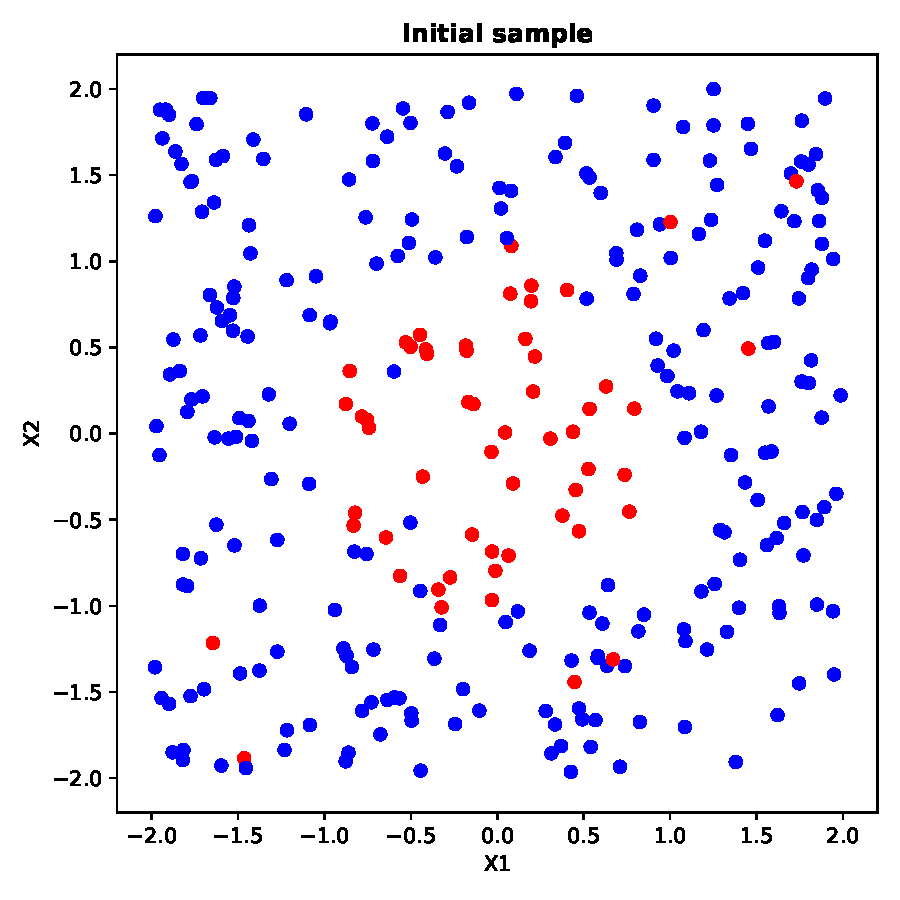
\includegraphics[width=0.4\textwidth]{images/svm_non_linear.pdf}
    \caption{Échantillon initial nécessitant une frontière de décision non-linéaire (ex: noyau radial)}
    \label{fig:svm_non_linear}
\end{figure}

Grâce à la dualité, on n'a pas besoin de connaître explicitement $\phi$, mais seulement la \textbf{fonction noyau} $K(x_i, x_j) = \phi(x_i) \cdot \phi(x_j)$. C'est le cœur du \textbf{Kernel Trick} (l'astuce du noyau) : \textbf{($\bigstar$ EXAMEN)} toute la mécanique du SVM (optimisation et décision) ne repose que sur les produits scalaires entre les observations. En substituant le produit scalaire standard par une fonction noyau $K$ adéquate (qui correspond mathématiquement à un produit scalaire dans $\mathbb{R}^P$), l'algorithme se comporte exactement \textit{comme s'il} projetait les points dans ce vaste espace, puis cherchait un hyperplan linéaire, le tout \textbf{sans jamais avoir à calculer explicitement les coordonnées} transformées $\phi(x)$, évitant ainsi un coût computationnel rédhibitoire ou infini.

\subsection{Noyaux Usuels}
\begin{itemize}
    \item \textbf{Polynomial :} $K(u, v) = (u^T v + 1)^\beta$.
    \item \textbf{Radial (RBF/Gaussien) :} $K(u, v) = e^{-\gamma \|u-v\|^2}$.
\end{itemize}
Un noyau doit satisfaire le \textbf{Théorème de Mercer} pour garantir qu'il définit un produit scalaire dans un espace de Hilbert.

\section{Extensions et Pratique}

\subsection{Multi-classes}
Comme le concept d'hyperplan est binaire ($K=2$), on utilise deux approches pour $K > 2$:
\begin{enumerate}
    \item \textbf{One-Versus-One (OVO) :} On entraîne $\frac{K(K-1)}{2}$ classifieurs pour chaque paire de classes. La classe gagnante est celle qui remporte le plus de duels.
    \item \textbf{One-Versus-All (OVA) :} On entraîne $K$ classifieurs (chaque classe contre toutes les autres). On choisit la classe avec le score le plus élevé.
\end{enumerate}

\subsection{Mise en œuvre avec R (package e1071)}
La fonction principale est \texttt{svm()}. \textbf{($\bigstar$ EXAMEN) Fait important pour la classification à plusieurs cibles :} cette fonction implémente par défaut l'approche \textbf{One-Versus-One (OVO)} pour la classification multi-classes.
\begin{itemize}
    \item \textbf{Scaling :} Il est crucial de centrer-réduire les prédicteurs pour éviter que les variables à forte échelle ne dominent.
    \item \textbf{Tuning et Hypéramètres :} 
    \begin{itemize}
        \item Le coût $C$ (\texttt{cost}) gère la tolérance aux violations de marge.
        \item Pour le noyau \textbf{Radial (Gaussien)}, \textbf{($\bigstar$ EXAMEN)} le paramètre \texttt{gamma} ($\gamma$) représente l'inverse de la taille de la fenêtre d'influence d'un vecteur support (la largeur du "creux" gaussien). Un $\gamma$ \textit{petit} signifie une large zone d'influence vis-à-vis du lissage (forte variance), tandis qu'un $\gamma$ \textit{fort} modélise un seuil très piqué conduisant le modèle à "épouser" chaque point (faible biais, très forte variance, sur-apprentissage probable).
    \end{itemize}
    La fonction \texttt{tune()} permet de sélectionner la meilleure combinaison de ces paramètres ($C$, $\gamma$) par validation croisée.
\end{itemize}

\begin{lstlisting}[caption=Exemple d'utilisation de e1071]
library(e1071)
# Ajustement d'un modele radial
svmfit <- svm(y ~ ., data=dat, kernel="radial", cost=10, gamma=1)
# Recherche des meilleurs parametres
tune.out <- tune(svm, y ~ ., data=dat, kernel="radial", 
                 ranges=list(cost=c(0.1,1,10,100), gamma=c(0.5,1,2)))
bestmod <- tune.out$best.model
\end{lstlisting}
